\chapter{Monte Carlo法:估算体积和计数}

这一章我们开始介绍Monte Carlo法的基础理论。从如何估算一个多维欧氏空间
中的有界区域的体积(Volumn)开始。更一般的问题则是在相同区域中估算积分。
当区域或目标函数复杂时,Monte Carlo法具有经典数值方法所无法取代的优势。
而计数估计(Evaluating count)则是另一个非常重要的问题。它的一个来源是
当我们有时需要估计一个元素数量为$m$的集合中具有指定性质的子集的个数。
但这种估算的经典算法往往是关于$m$指数增长的。也即我们无法精确地列举全
部子集,然后进行计数。Monte Carlo法在这种情形下,也具有优势。

尽管体积估算和计数估计一个是连续,一个是离散。但实际上这是一类基础问题
的不同方面。它们实际上的理论和技巧是相通的。甚至我们有时直接将计数包含
进体积的概念之中以简化叙述。

\section{体积估计}

令$\mathscr{R}$是一个包含在$m$维超立方体
\begin{equation}
  \mathscr{J}^m = [0, 1]^m = [0, 1] \times \cdots \times [0, 1]
  \label{eq::hyper_cube}
\end{equation}
中的$m$维有界区域,且其体积$\lambda(\mathscr{R})$未知。而对于一般的有
界区域,我们假设可以通过适当的变换将其映射进$\mathscr{J}^m$。如果我们
能够产生$m$维点列
\begin{equation}
  \mathscr{K}_{m, n} = \left\{\vec{x}^{(j)} = (x_1^{(j)}, x_2^{(j)},
  \cdots, x_m^{(j)}) \in \mathscr{J}^m, j = 1, \cdots, n\right\},
  \label{eq::m_d_random_number}
\end{equation}
则$\lambda(\mathscr{R})$可以用$\bar{\lambda}_n(\mathscr{R})$来逼近。伪
代码如算法\ref{alg::volumn}。

\begin{minipage}[!ht]{0.8\textwidth}
\vspace{3ex}
\refstepcounter{alg}
\label{alg::volumn}
\begin{center}
 算法 \arabic{chapter}.\arabic{alg} 估算体积
\end{center}
\small
\begin{tabular}{ll}
  \hei 目标&估算$\lambda(\mathscr{R})$.\\
  \hei 输入&包含在$\mathscr{J}^m$中的区域$\mathscr{R}$, 以及$n$个计值点.\\
  \hei 输出&$\bar{\lambda}_n(\mathscr{R})$.
\end{tabular}
\begin{enumerate}
\item $j = 1$, $S = 0$.
\item While $j \leq n$:
  \begin{enumerate}
    \item 从$\mathscr{K}_{m, n}$中产生$\vec{x}^{(j)}$.
    \item $\phi(\vec{x}^{(j)}) = 0$.
    \item If $\vec{x}^{(j)} \in \mathscr{R}, \phi(\vec{x}^{(j)}) = 1$.
    \item $S = S + \phi(\vec{x}^{(j)})$.
    \item j = j + 1.
  \end{enumerate}
  \item 计算$\bar{\lambda}_n(\mathscr{R}) = S/n$.
\end{enumerate}
\end{minipage}

这里具体的$\bar{\lambda}(\mathscr{R})$的数值精度依赖$\mathscr{R}$和
$\mathscr{K}_{m, n}$的性质。比如如果取均匀划分的网格点,则有
\begin{equation}
  \mathscr{K}_{m, n} = \left\{\vec{x} = (x_1, \cdots, x_m) : x_i =
  \frac{z_i + \frac{1}{2}}{k}, z_i = 0, \cdots, k - 1, i = 1, \cdots,
  m, n = k^m\right\}.
  \label{eq::m_d_lattice}
\end{equation}
这个公式的含义是格点在第$i$维的坐标$x_i$可以取$z_i = 0, \cdots, k - 1$
中的任何一个,可以重复取,这样的组合一共有$n = k^m$个,每一组都代表了
一个$m$维超单位正方体$\mathscr{J}^m$中的均匀格点。比如我们不难画出2维
的特例(见图\ref{fig::2_d_lattice})。可以看到$k$代表了在一个维度上的均匀格点个数。每一个格点,均是
一个体积为$1 / k^m = 1 / n$的小超正方体的中心。因此落在
$\mathscr{R}$内的格点个数$S$可以估算出$\mathscr{R}$的体积
$$
\lambda(\mathscr{R}) \approx \bar{\lambda}_n(\mathscr{R}) =
\frac{S}{n}.
$$

\begin{figure}[!ht]
\centering
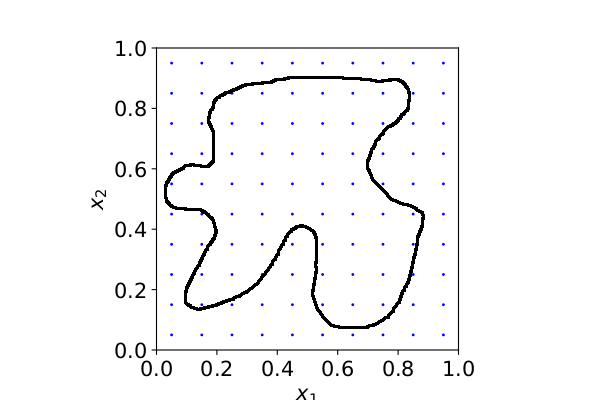
\includegraphics[width=0.7\textwidth]{images/lattice.png}
\caption{二维单位正方体内的均匀网格,$k = 10$。中间不规则区域表示$\mathscr{R}$。}
\label{fig::2_d_lattice}
\end{figure}

如果我们用$s(\mathscr{R})$表示二维区域$\mathscr{R}$的边长,那么通过观
察不难看出绝对误差有上界估计
\begin{equation}
  \left|\bar{\lambda}_n(\mathscr{R}) - \lambda(\mathscr{R})\right|
  \leq \frac{s(\mathscr{R})}{k}.
  \label{eq::2_d_absolute_error}
\end{equation}
事实上,包含了不确定的绝对误差部分最大不会超过长度为$s(\mathscr{R})$,
宽度为$1/k$的条状地带面积。而更一般的,如果用$s(\mathscr{R})$表示一个
$m$维区域$\mathscr{R}$的表面积,则对应的绝对误差界也是
(\ref{eq::2_d_absolute_error})。由$n = k^m$,有
\begin{equation}
  \left|\bar{\lambda}_n(\mathscr{R}) - \lambda(\mathscr{R})\right|
  \leq \frac{s(\mathscr{R})}{n^{\frac{1}{m}}},
  \label{eq::m_d_absolute_error}
\end{equation}
也即误差收敛率随$m$上升而下降。或者说,如果要保证误差小于$\varepsilon \in (0, 1)$,则
需要
$$
n(\varepsilon) =
\left\lceil\left(\frac{s(\mathscr{R})}{\varepsilon}\right)^m\right\rceil
$$
个点才能保证。

而Monte Carlo方法只改变其中一步,即将序列$\{\vec{x}^{(1)}, \cdots,
\vec{x}^{(n)}\}$从一个确定的序列,改成一系列在$\mathscr{J}^m$中均匀分
布的独立随机变量
$$
\vec{X}^{(j)} = \{X_1^{(j)}, \cdots, X_m^{(j)}\}, j = 1, \cdots, n.
$$也即,$X_i$的PDF均为$U(0, 1)$. 做相应修改后的算法\ref{alg::volumn}就
是Monte Carlo算法,简称MC,或者,也称作标准Monte Carlo采样(standard
Monte Carlo sampling)。我们用算法\ref{alg::MC}表示。

\begin{minipage}[!ht]{0.8\textwidth}
\vspace{3ex}
\refstepcounter{alg}
\label{alg::MC}
\begin{center}
 算法 \arabic{chapter}.\arabic{alg} MC
\end{center}
\small
\begin{tabular}{ll}
  \hei 目标&估算$\lambda(\mathscr{R})$.\\ \hei 输入&包含在
  $\mathscr{J}^m$中的区域$\mathscr{R}$, 样本尺寸$n$, 置信水平$1 -
  \delta$. \\
  \hei 输出&估计值$\bar{\lambda}_n(\mathscr{R})$, 方差$\mathrm{var} \bar{\lambda}_n(\mathscr{R})$ 以及置信区间.
\end{tabular}
\begin{enumerate}
\item $j = 1$, $S = 0$.
\item While $j \leq n$:
  \begin{enumerate}
    \item 生成$\vec{X}^{(j)}$.
    \item $\phi(\vec{X}^{(j)}) = 0$.
    \item If $\vec{X}^{(j)} \in \mathscr{R}, \phi(\vec{X}^{(j)}) = 1$.
    \item $S = S + \phi(\vec{X}^{(j)})$.
    \item j = j + 1.
  \end{enumerate}
\item 做统计分析:
  \begin{enumerate}
  \item 计算$\bar{\lambda}_n(\mathscr{R}) = S/n$作为$\lambda(\mathscr{R})$的点估计.
  \item 计算$V[\bar{\lambda}_n(\mathscr{R})] = (S / n)(1 - S / n) / (n - 1)$ 作为$\mathrm{var~} \bar{\lambda}_n(\mathscr{R})$的点估计.
  \item 根据置信水平计算百分之$100 \times (1 - \delta)$的置信区间.
  \end{enumerate}
\end{enumerate}
\end{minipage}

注意到$\vec{X}^{(1)}, \cdots \vec{X}^{(n)}$均为独立随机变量且PDF为
\begin{equation}
  f(\vec{x}) = \left\{
  \begin{array}{ll}
    1, & 0 \leq x_i \leq 1, i = 1, \cdots, m,\\
    0, & \mbox{其他}.
  \end{array}
  \right.
  \label{eq::MC_X_PDF}
\end{equation}
因此$\phi(\vec{X}^{(1)}), \cdots, \phi(\vec{X}^{(n)})$为独立的
Bernoulli分布随机变量,满足
\begin{equation}
  P\{\phi(\vec{X}^{(j)}) = 1\} = \int_{\mathscr{R}} f(\vec{x}) dx =
  \lambda(\mathscr{R})
  \label{eq::MC_phi_X}
\end{equation}
且
\begin{equation}
  P\{\phi(\vec{X}^{(j)}) = 0\} = \int_{\mathscr{J}^m \backslash
    \mathscr{R}} f(\vec{x}) dx = 1 - \lambda(\mathscr{R}), j = 1, \cdots, n.
  \label{eq::MC_phi_X_R}
\end{equation}
所以,$S = \phi(\vec{X}^{(1)}) + \cdots + \phi(\vec{X}^{(n)})$服从二项分布
\begin{equation}
  P\{S = i\} = f_i(n, \lambda) = \binom{n}{i} \lambda^i (1 -
  \lambda)^{(n - i)}, \lambda = \lambda(\mathscr{R}), i = 0, \cdots, n.
  \label{eq::MC_Bernoulli}
\end{equation}
二项分布的期望和方差分别是$E[S] = n \lambda$和$\mathrm{var~} S =
n\lambda(1 - \lambda)$. 于是$\bar{\lambda}_n =
\bar{\lambda}_n(\mathscr{R})$可以看作是$\lambda$的一个无偏估计,且有
\begin{equation}
  \mathrm{var~} \bar{\lambda}_n = \frac{1}{n^2} \mathrm{var~} S =
  \lambda (1 - \lambda) / n.
  \label{eq::var_lambda_bar}
\end{equation}
注意其实$\lambda$是未知量,因此我们并不能用公式(\ref{eq::var_lambda_bar})来估算误差。

\section{误差和样本大小}

首先我们要明确,对Monte Carlo法而言,收敛指的是依概率$1$收敛,也即
\begin{equation}
  P\left\{\lim_{n \to \infty} \bar{\lambda}_n = \lambda \right\} = 1.
\end{equation}
因此,所谓误差也是点估计或区间估计意义上的。比如算法\ref{alg::MC}中的
$V[\bar{\lambda}_n(\mathscr{R})]$就是$\mathrm{var~} \bar{\lambda}_n$的
一个无偏估计,因为
\begin{equation}
  \begin{array}{rcl}
  E[(S / n) (1 - S / n)] &=&  \displaystyle \frac{1}{n} E[S] -
  \frac{1}{n^2}(\mathrm{var~} S + E^2[S])\\\\
  &=& \displaystyle\frac{\lambda (1 - \lambda) (n - 1)}{n}.
 \end{array}
\end{equation}

而$\sqrt{V[\bar{\lambda}_n]}$被称为$\bar{\lambda}_n$的标准误差(standard
  error)。有时被用作$\bar{\lambda}_n$的统计误差的一个粗略估计,不过由
于$V[\bar{\lambda}_n]$本身就是一个估计量,因此要慎重使用。要系统考虑误
差的分布,则需要统计学理论,我们陆续会选择一些重要的(或者对我们而言有
  用的)介绍。

\begin{theorem}{\hei \bf Chebshev不等式}
  令$Z$是一个累积分布为$F(z)$的随机变量,$z \in (-\infty, \infty)$。且$E[Z] = 0$,
  $\sigma^2 = \mathrm{var~} Z = E[Z^2] < \infty$。则对$\beta > 0$,有
  \begin{equation}
    P\left\{\frac{|Z|}{\sigma} \geq \beta\right\} \leq \frac{1}{\beta^2}.
    \label{eq::cheb_ineq}
  \end{equation}
  \label{thm::cheb_ineq}
\end{theorem}

\begin{proof} 对$\varepsilon > 0$,有
  \begin{equation}
    \begin{array}{rcl}
    P\{|Z| \geq \varepsilon\} &=& \displaystyle
    \int_{-\infty}^{-\varepsilon}d F(z) + \int_{\varepsilon}^{\infty}d
    F(z) \\\\ &\leq& \displaystyle
    \int_{-\infty}^{-\varepsilon}\frac{z^2}{\varepsilon^2} d F(z)
    + \int_{\varepsilon}^{\infty}\frac{z^2}{\varepsilon^2} d F(z)\\\\
    &\leq& \displaystyle \frac{1}{\varepsilon^2}\int_{-\infty}^{\infty}z^2 d F(z)
    = \frac{\sigma^2}{\varepsilon^2}.
    \end{array}
  \end{equation}
  取$\beta = \varepsilon / \sigma$即得(\ref{eq::cheb_ineq})。
\end{proof}

现取$Z = S / n - \lambda$和$\sigma^2 = \lambda(1 - \lambda) / n$,得
\begin{equation}
  P\{|\bar{\lambda}_n - \lambda| < \varepsilon\} \geq 1 - \lambda(1 - \lambda) / n \varepsilon^2.
  \label{eq::col_cheb_ineq}
\end{equation}
即
\begin{equation}
  \lim_{n \to \infty} P\{|\bar{\lambda}_n - \lambda| \geq \varepsilon\} = 0.
  \label{eq::cov_pro}
\end{equation}
上式称为概率收敛(convergence in probability),由依概率1收敛可以导出
概率收敛,但反过来不行。它比依概率1收敛(convergernce with 
  probability 1,缩写w.p.1)要弱。但这里实际给出了一个收敛性和样本大小$n$之
间的关系。不过这里再大的$n$都不能\CJKunderdot{确保}误差小于
$\varepsilon$。为了正确的体现和评估随机性,我们需要引入置信水平
(confidence level)$1 - \delta$,$0 < \delta < 1$,由Chebyshev不等式,
当
\begin{equation}
  n \geq n_C(\varepsilon, \delta, \lambda) = \lceil \lambda (1 -
  \lambda) / \delta \varepsilon^2 \rceil
  \label{eq::cheb_ineq_est}
\end{equation}
时,误差满足
\begin{equation}
  P\{|\bar{\lambda}_n - \lambda| < \varepsilon\} \geq 1 - \delta.
  \label{eq::abs_error_crit}
\end{equation}
我们称其为绝对误差准则(absolute error criterion)。注意到$\lambda(1 -
\lambda) \leq 1 / 4$,故有最坏情形样本数(the worst-case sample size)
\begin{equation}
  n_C(\varepsilon, \delta) = \lceil \frac{1}{4 \delta \varepsilon^2}\rceil,
  \label{eq::wc_sample_s}
\end{equation}
对所有$\lambda \in [0, 1]$。

公式(\ref{eq::wc_sample_s}) 表达了Monte Carlo法最重要的性质,
$n_C(\varepsilon, \delta, \lambda)$和维数$m$无关。而在实际计算中,由于
随机投点本身是一个$O(m)$的操作,且在每个维度上我们要通过计算来判断
$\vec{X}$是否属于$\mathscr{R}$,这些操作加起来不超过$O(m^\beta)$,
$\beta \geq 1$。故实际在程序中估算绝对误差界的代价是
$$
O([m^\beta \frac{\lambda (1 - \lambda)}{\delta \varepsilon^2}])
= O(\frac{m^\beta}{4 \delta \varepsilon^2}).
$$
仍然是一个关于$m$的多项式时间算法,而相应精确逼近算法关于$m$是指数时间的。

尽管公式(\ref{eq::wc_sample_s})给出了一个样本数的估计,但这个估计明
显是过宽的。实际上的样本数需求要远小于这个估计。为此我们考虑根据中心极
限定理,当$n \to \infty$时,特征量
$$
\frac{S - n \lambda}{[n \lambda (1 -
  \lambda)]^{\frac{1}{2}}}
$$
是服从标准正态分布
\begin{equation}
  \Phi(z) = (2 \pi)^{-\frac{1}{2}}\int_{-\infty}^z e^{-\frac{y^2}{2}} dy, -\infty < z < \infty,
  \label{eq::cdf_std_normal}
\end{equation}
也即$N(0, 1)$分布。令
\begin{equation}
  n_N(\varepsilon, \delta, \lambda) = \left\lceil \lambda (1 -
  \lambda) \left[\frac{\Phi^{-1}(1 -
      \frac{\delta}{2})}{\varepsilon}\right]^2\right\rceil,
  \label{eq::es_sample_s}
\end{equation}
其中
\begin{equation}
  \Phi^{-1}(\theta) = \inf\left[z : (2 \pi)^{-\frac{1}{2}}
    \int_{-\infty}^z e^{-\frac{y^2}{2}} dy = \theta, 0 < \theta < 1\right].
\end{equation}
于是当$\varepsilon \to 0$, 公式(\ref{eq::es_sample_s})给出了在参数
$(\varepsilon, \delta)$下,绝对误差满足
\begin{equation}
  \lim_{\varepsilon \to 0} P\left\{\frac{\left|\frac{S}{n_N(\varepsilon,
      \delta, \lambda)} - \lambda\right|}{\varepsilon} \leq 1\right\} = 1 - \delta
  \label{eq::es_pro_abs_error}
\end{equation}
的样本数。而对应的最坏情形样本数是
\begin{equation}
  n_N(\varepsilon, \delta) = \left\lceil \left[\frac{\Phi^{-1}(1 -
      \frac{\delta}{2})}{2\varepsilon}\right]^2\right\rceil.
  \label{eq::es_worst_sample_s}
\end{equation}

我们可以比较在$\delta = 0.001$, $0.01$和$0.05$下,
$$
\frac{n_C}{n_N} = \frac{1}{\delta\left[\Phi^{-1}(1 - \frac{\delta}{2})\right]^2}
$$的值分别是$92.36$, $15.07$和$5.21$。可见这个比例还是很大的。不过这么
估计也有比较严重的问题。因为我们实际上就把$S / n$当作正态分布计算了,
而这个只是一个概率极限情形。因此,当$n$不够大(注意这里逻辑上有矛盾),
或者$\varepsilon$太小时,这个结果都有很大的误差。一个弥补的办法是故意
高估$n$,比如有人建议总是取两倍的$n_N$。而更加靠谱的估计,来自
Hoeffding于1963年的工作\cite{Wassily1963Probability}。(以下部分只要了
  解结论,不作要求。)

\begin{theorem}{\bf Hoeffding 1963}
  令$Z_1, \cdots, Z_n$是独立随机变量且
  $$
  \mu_i = E[Z_i] \in (0, 1), P\{0 \leq Z_i \leq 1\} = 1, i = 1, \cdots, n.
  $$
  令$\mu = (\mu_1 + \cdots + \mu_n) / n$。 则对$0 < \varepsilon < 1 -\mu$,和
  $\bar{Z}_n = (Z_1 + \cdots + Z_n) / n$,
  \begin{eqnarray}
    P\{\bar{Z}_n - \mu \geq \varepsilon\} &\leq& e^{n w(\varepsilon, \mu)} \\
    \label{eq::hoeffding1963_1}
    & \leq & e^{-\mu g(\mu) \varepsilon^2} \\
    \label{eq::hoeffding1963_2}
    & \leq & e^{-2 n \varepsilon^2},
    \label{eq::hoeffding1963_3}
  \end{eqnarray}
  其中
  \begin{equation}
    w(\varepsilon, \mu) = (\mu + \varepsilon) \log
    \left(\frac{\mu}{\mu + \varepsilon}\right) + (1 - \mu -
    \varepsilon) \log\left(\frac{1 - \mu}{1 - \mu - \varepsilon}\right),
    \label{eq::hoeffding1963_w}
  \end{equation}
  以及
  \begin{equation}
    g(\mu) =
    \left\{
        \begin{array}{ll}
          \displaystyle \frac{1}{1 - 2 \mu} \log\left(\frac{1 -
            \mu}{\mu}\right),& \mbox{若} 0 < \mu <
          \frac{1}{2}\\\\ \displaystyle \frac{1}{2\mu(1 - \mu)},&
          \mbox{若} \frac{1}{2} \leq \mu < 1.
        \end{array}\right.
        \label{eq::hoeffding1963_g}
  \end{equation}
  \label{thm::Hoeffding1963}
\end{theorem}

\begin{corollary}
  对公式(\ref{eq::hoeffding1963_w})中定义的$w(\varepsilon, \mu)$,
  \begin{equation}
    \lim_{\varepsilon \to 0} \varepsilon^{-2} w(\varepsilon, \mu) =
    -\frac{1}{2\mu(1 - \mu)}。
  \end{equation}
  \label{cor::hoeff_1}
\end{corollary}

\begin{corollary}
  函数$w(\varepsilon, y)$,$0 < \varepsilon < 1 - y$,$0 < y < 1$关于
  $y$是凹的。故有最大值$y^* \in [\max(0, \frac{1}{2} - \varepsilon),
    \frac{1}{2}]$。
  \label{cor::hoeff_2}
\end{corollary}

\begin{corollary}
  函数$w((y + v)\varepsilon, y)$,$0 < \varepsilon \leq \frac{1 - y}{y
    + v}$,$0 < y < 1$,$v \geq 0$;和函数$w((y + v)\varepsilon, 1 -
  y)$,$0 < \varepsilon \leq \frac{y}{y + v}$,$0 < y < 1$,$v > 0$,
  关于$y$都是凹的。
  \label{cor::hoeff_3}
\end{corollary}

\begin{corollary}
  对公式(\ref{eq::hoeffding1963_w})中定义的$w(\varepsilon, y)$,有
  $w(\varepsilon, y) \geq w(\varepsilon, 1 - y)$,$\varepsilon \leq y
  \leq \frac{1}{2}$。
  \label{cor::hoeff_4}
\end{corollary}

以上证明略。自行参考\cite{Fishman1995Monte}第24页、附录及Hoeffding原文。
该定理可导出一系列有用的结论。比如样本量的估计:
\begin{equation}
  n_H(\varepsilon, \delta) =
  \left\lceil\frac{2\log(\frac{2}{\delta})}{4\varepsilon^2}\right\rceil.
  \label{eq::hoeff_sample_no_1}
\end{equation}
以及对$\varepsilon < \min\{\mu, 1 - \mu\}$(这里$\mu = \lambda$),有
\begin{equation}
  n_H(\varepsilon, \delta) =
  \left\lceil\frac{\log(\frac{\delta}{2})}
                   {\sup_{\varepsilon \leq v \leq 1 - \varepsilon} w(\varepsilon, v)}
                   \right\rceil.
  \label{eq::hoeff_sample_no_2}
\end{equation}
这里公式(\ref{eq::hoeff_sample_no_2})分母中的最大值可以用数值方法求
解。这两个估计一般认为是比$n_N$更精确的估计。

\section{置信区间}

之前我们给出了面积的一个点估计$\bar{\lambda}_n$,以及讨论在置信度
$\delta$下的一个关于偏差$\varepsilon$的样本数量估计。似乎所有关于计算
模拟的信息已经具备了,为何还要继续讨论区间估计呢?或者说区间估计难道不
就是
$$
P\{|\bar{\lambda}_n - \lambda| \leq \varepsilon\} = 1 - \delta
$$
吗?这个结果有两个比较可疑的地方,一个是这个区间居然是对称的;另一个是
这个估计居然和$\lambda$无关。
%% 我们倒是学过另一个点估计值
%% $V[\bar{\lambda}_n]$,并称它的算术平方根为标准误差,作为一个误差的估计。
%% 我们注意到它也是对称的,但它和$S$,进而和$\lambda$有关。通过我们的作业,
%% 我们了解到$\sqrt{V[\bar{\lambda}_n]}$和$\bar{\lambda}_n$具有相关性,也就
%% 是$\bar{\lambda}_n$越接近$0$,$\sqrt{V[\bar{\lambda}_n]}$会越小;
%% $\bar{\lambda}_n$越接近$1$,$\sqrt{V[\bar{\lambda}_n]}$会越大。而且这种趋
%% 势,无法通过增加$n$消除。这一点我们可以通过概率论的推导证明。
但是我们考虑一下如果一个实际的$\lambda$比较接近$0$,那么在随机投点时,
落入$\mathscr{R}$内的点数本身就相对有限,因此其频率$\bar{\lambda}_n$往
负方向\CJKunderdot{可能的}偏差就很有限。比如$\lambda = 0.005$,那么负
方向的偏差不可能大于$0.005$。但正方向的偏差却仍然服从方差分布的规律,
可以大于$0.005$。于是我们应该能观察到频率$\bar{\lambda}_n$的分布往正方
向偏的现象。图(\ref{fig::bias_lambda_n})给出了$n = 1000$时,对一个面
积为$0.005$的圆进行Monte Carlo求面积时的频率分布的统计,总共做了
$50000$组实验。我们可以看到,实际的频率分布确实是往正方向偏移的。因为
负方向根本没有偏移的空间了。

\begin{figure}[!ht]
\centering
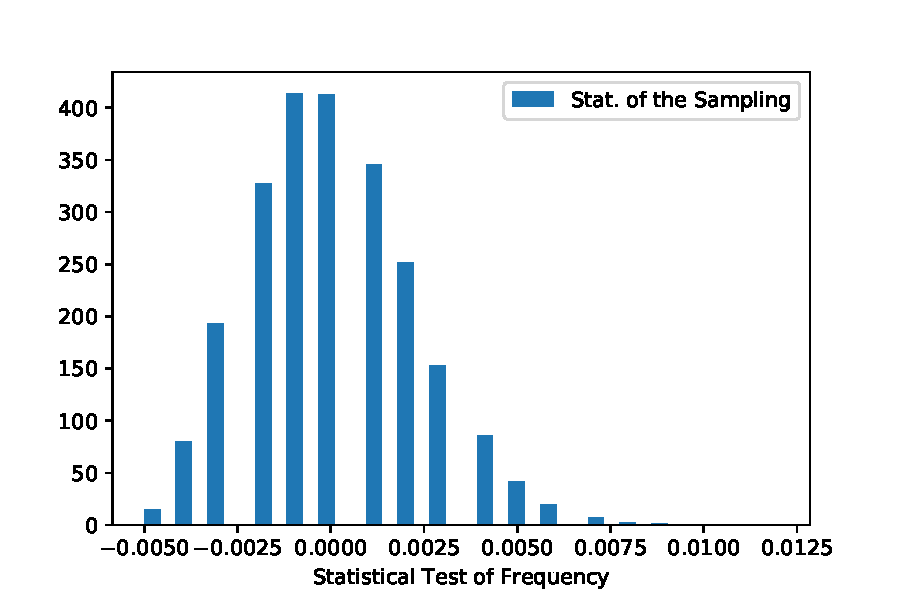
\includegraphics[width=0.7\textwidth]{images/bais_lambda_n.pdf}
\caption{对一个面积为$0.005$的圆进行Monte Carlo求面积时频率分布的统计,
  $n = 1000$,总共做了$50000$组实验。}
\label{fig::bias_lambda_n}
\end{figure}

以上这些观察提示我们,实际频率的分布和频率本身有关,同时也应该有一定的
偏移。这就是区间估计的出发点。我们希望将频数$S$也纳入统计估计,给出一
个置信区间的上下界范围。也即寻找$I_1 = I_1(S, n, \delta)$和$I_2 =
I_2(S, n, \delta)$,使得
$$
P\{I_1, I_2, \delta\} = P\{I_1 < \lambda < I_2\} \geq 1 -\delta.
$$
这里$P\{I_1, I_2, \delta\}$称为范围概率(coverage probability)或者可
靠系数(confidence coefficent)。而区间$[I_1, I_2]$称为置信区间
(confidence interval)。置信区间是比给出一个单点估计$\bar{\lambda}_n$
更加可靠的统计估计。关于二项分布的区间估计的理论和方法很多。我们这里给
出三种主要方法。

记二项分布的累计分布函数为
\begin{equation}
  F_i(n, \mu) = \sum_{j = 0}^i \binom{n}{j} \mu^j (1 - \mu)^{n - j}, 0
  < \mu < 1, i = 0, 1, \cdots, n.
  \label{eq::binomial_CDF}
\end{equation}
因此对$0 < \alpha_1 < \alpha_2 <1$,存在唯一的$\theta_1(s, n, \alpha_1)$和
$\theta_2(s, n, \alpha_2)$分别满足
\begin{equation}
  1 - F_{s - 1}(n, \theta) = \alpha_1
  \label{eq::binomial_theta_1}
\end{equation}
和
\begin{equation}
  F_s(n, \theta) = 1 - \alpha_2.
  \label{eq::binomial_theta_2}
\end{equation}
特别地,对$s = 1$,我们分别令$\theta_1 = 0$和$\theta_2 = 1$。注意到
$F_s(n, \theta)$关于$\theta$递减和关于$s$递增,所以有
$$
0 \leq \theta_1(s, n, \alpha_1) < \theta_2(s, n, \alpha_2) \leq 1.
$$
因此,若对$n$次独立的Bernolli试验,恰好成功$S$次的概率是$\mu$,则对满足
$$
1 + \alpha_1 - \alpha_2 = \delta
$$
的$\alpha_1$和$\alpha_2$,而区间$[\theta_1(S, n, \alpha_1),
  \theta_2(S, n, \alpha_2)]$就是$\mu$关于置信水平$\delta$的范围区间,也即
$$
P\{\theta_1(S, n, \alpha_1) < \mu < \theta_2(S, n, \alpha_2)\} \geq 1 - \delta.
$$
满足上面条件的$\alpha_1$和$\alpha_2$很多,我们这里采用的是$\alpha_1
= \frac{\delta}{2}$和$\alpha_2 = 1 - \frac{\delta}{2}$. 也即我们最终取
$$
I_1(S, n, \delta) = \theta_1(S, n, \frac{\delta}{2}),
I_2(S, n, \delta) = \theta_2(S, n, 1 - \frac{\delta}{2}).
$$

为了计算$\theta_1$和$\theta_2$,我们引入不完全Beta函数\cite{Abramowitz1970Handbook}:
\begin{equation}
  1 - F_{j - 1}(n, \theta) = H_\theta(j, n - j + 1) = \frac{1}{B(j, n
    - j + 1)}\int_0^\theta z^{j - 1}(1 - z)^{n - j} dz, 0 \leq \theta \leq 1.
  \label{eq::incomplete_beta}
\end{equation}
其中$B(\cdot, \cdot)$表示Beta函数。而$H_\theta(j, n - j + 1)$实际上就
是参数为$j$和$n - j + 1$的Beta分布的累积分布函数。而所求
$$
\theta_1(S, n, \frac{\delta}{2}), \theta_2(S, n, 1 - \frac{\delta}{2})
$$
就分别是方程
$$
H_\theta(S, n - S + 1) = \frac{\delta}{2},
H_\theta(S + 1, n - S) = 1 - \frac{\delta}{2}
$$
的根。

在具体求根的时候,注意到$H_\theta$关于$\theta$的单调性,我们可以用二分
法来求解。初始含根区间可以选为$\theta_a = 0$,$\theta_b = 1$。如果要加
速收敛,可以在误差达到一定精度后采用Newton迭代。这些方法是经典数值方法,
这里不再详述,具体例子可参见讲义第四章附带代码。表
\ref{table::confidence_intervals}给了一些实际计算的结果做参考。

 \begin{table}[!ht]
   \centering
   \caption{置信区间举例,$n = 1000$,$1 - \delta = 0.99$。其中
     $H_1 = H_\theta(S, n - S + 1, \theta_1)$,
     $H_2 = H_\theta(S + 1, n - S, \theta_2)$。}
   \label{table::confidence_intervals}
\begin{tabular}{|c|c|c|c|c|c|c|}
  \hline
  $S$ & $\bar{\lambda}_n$ & $\theta_1$ & $\theta_2$&
  $H_1$&$H_2$&
  $P\{\theta_1 < \lambda < \theta_2\}$\\
  \hline
  11&0.0011&0.004334&0.02265& 0.005003&0.99501&0.990007\\
  \hline
\end{tabular}
\end{table}

第二种置信区间的求法可以总结成一个定理:


\begin{theorem}{}
  令$S$有均值$n \lambda$和方差$n \lambda(1 - \lambda)$,定义
  \begin{equation}
    \omega_i(z, n, \beta) = \frac{z + \frac{\beta^2}{2} +
      \beta(-1)^i\sqrt{\frac{\beta^2}{4} + \frac{z(n - z)}{n}}}{n +
      \beta^2}
    \label{eq::conf_int2}
  \end{equation}
  其中$\beta > 0$,$n \in \mathbb{N}^+$,$0 \leq z \leq n$并且$i = 1,
  2$。则存在$\beta = \beta(\delta)$使得开区间$(\omega_1(S, n, \beta),
  \omega_2(S, n, \beta))$以概率$\geq 1 - \delta$覆盖了$\lambda$。
  \label{thm::conf_int2}
\end{theorem}

\begin{proof}
  由Chebshev不等式,
  \begin{equation}
    P\left\{\frac{\left|\frac{S}{n} - \lambda\right|}{\sqrt{\lambda(1
        - \lambda)}} < \beta\right\} = P\left\{(\frac{S}{n} -
    \lambda)^2 < \frac{\beta^2 \lambda (1 - \lambda)}{n}\right\} \leq
    1 -\frac{1}{\beta^2},
    \label{eq::proof_conf_int2}
  \end{equation}
  所以只要取$\beta = \frac{1}{\sqrt{\delta}}$即得:
  \begin{equation}
    P\left\{\left[\omega_1(S, n \frac{1}{\sqrt{\delta}}) -
      \lambda\right]\left[\omega_2(S, n, \frac{1}{\sqrt{\delta}}) -
      \lambda\right] < 0\right\} \geq 1 - \delta.
  \end{equation}
\end{proof}

我们知道,Chebyshev不等式是过宽估计的,所以我们一般实际取
$$
\beta = \Phi^{-1}(1 - \frac{\delta}{2}), 0 < \lambda < 1,
$$
然后令$I_1(S, n, \delta) = \omega_1(S, n, \beta)$和$I_2(S, n,
\delta) = \omega_2(S, n, \beta)$。

不过基于正态分布的$\beta$估值,同样会导致在$\lambda$接近$0$或$1$时,置
信区间覆盖不住$\lambda$。通过修正
\begin{equation}
  \bar{\omega}_i(z, n, \beta) = \omega_i(z + 0.5 \times (-1)^i, n,
  \beta), i = 1, 2.
  \label{eq::con_corr}
\end{equation}
一般在$\lambda < 0.3$或$\lambda > 0.7$,实际操作中,发现$S$小于$0.3n$
或大于$0.7n$时,可以考虑做此修正。具体理论分析参见\cite{Blyth1983Binomial}。

第三种置信区间估计不再依赖具体的分布,它也可以总结成一个定理。首次发表
人就是我们参考书的作者。

\begin{theorem}{\hei Fishman 1991}
  令$Z_1$,$\cdots$,$Z_n$为独立随机变量,且$\mu = E[Z_i] \in (0, 1)$,
  $P\{0 \geq Z_i \geq 1\} = 1$,令
  $$
  \bar{Z} = \frac{Z_1 + \cdots + Z_n}{n},
  $$
  对$0 \leq z \leq 1$和$0 < \delta < 1$,定义
  \begin{equation}
    \rho_1(z, n, \delta) = \left\{ \begin{array}{ll}
      \{t : 0 < t \leq z \leq 1, e^{n w(z - 1, t)} = \frac{\delta}{2} \}& z > 0\\
      0 & z = 0.
      \end{array}
      \right.
      \label{eq::conf_int3_rho_1}
    \end{equation}
    和
    \begin{equation}
      \rho_2(z, n, \delta) = \left\{ \begin{array}{ll}
      \{t : 0 < t \leq z \leq 1, e^{n w(t - z, 1 - t)} = \frac{\delta}{2} \}& z < 1\\
      0 & z = 1.
      \end{array}
      \right.
      \label{eq::conf_int3_rho_1}
      \end{equation}
      其中$w$的定义如(\ref{cor::hoeff_3})。则
      $$
      P\{\rho_1(\bar{Z}_n, n, \delta) < \mu < \rho_2(\bar{Z}_n, n, \delta)\} \geq 1 - \delta.
      $$
    \label{thm::conf_int3}
\end{theorem}

具体应用时,取$I_1(S, n, \delta) = \rho_1(frac{S}{n}, n, \delta)$和
$I_2(S, n, \delta) = \rho_2(\frac{S}{n}, n, \delta)$。在求解过程中,需
要关于$w$的方程,可以用和之前一样的求根技巧。以上三个方法,请大家自行
编写代码验证,这里给出一些结果供对比。

\begin{table}[!ht]
   \centering
   \caption{置信区间举例,$n = 1000$,$1 - \delta = 0.99$。}
   \label{table::confidence_intervals_2}
\begin{tabular}{|c|c|c|c|c|c|c|c|}
 \hline
 $S$ & $\bar{\lambda}_n$ & $\omega_1$ & $\omega_2$&
 $\bar{\omega}_1$&$\bar{\omega}_2$&
 $\rho_1$&$\rho_2$\\
 \hline
 11&0.0011&0.005163&0.02328&0.004844&0.02396&0.003421&0.02540\\
 \hline
 323&0.2862&0.3622&0.2857&0.3627&0.2762&0.3723&0.02540\\
 \hline
\end{tabular}
\end{table}

我们这里介绍的只是误差估计的非常基础的部分,更深入的理论和分析需要更专
业的统计学知识,大家可参阅相关资料。参考书2.4-2.5章也提供了更多的讨论。
我们在这一节最后集中讨论一下一个在计算机模拟中常见的策略。如果存在
$\mathscr{R}$的超矩形下界$\mathscr{R}_L$和上界$\mathscr{R}_U$(在二维
  可以想像成一个内接矩形和一个外接矩形),那么我们的随机投点范围可以缩
小,从而提高算法效率。这里可令
\begin{equation}
  \mathscr{R}_{L} = \{\vec{x} \in \mathscr{J}^m : 0 \leq \alpha_{Li} \leq x
  \leq \beta_{Li} \leq 1, 1 \leq i \leq m\}
\end{equation}
和
\begin{equation}
  \mathscr{R}_{U} = \{\vec{x} \in \mathscr{J}^m : 0 \leq \alpha_{Ui} \leq x
  \leq \beta_{Ui} \leq 1, 1 \leq i \leq m\}
\end{equation}
并且,对$\forall \vec{x} \in \mathscr{J}^m$,如果$\vec{x} \in
\mathscr{R}_L$,则必有$\vec{x} \in \mathscr{R}$;如果$\vec{x} \in
\mathscr{J}^m \backslash \mathscr{R}_U$,则必有$\vec{x} \notin
\mathscr{R}$.图\ref{fig::hyperrectangle2D}给出了一个二维的例子(俺先盗个图)。
注意到$\mathscr{R}_L$和$\mathscr{R}_U$的体积分别为
\begin{equation}
  \lambda_L = \prod_{i = 1}^m(\beta_{Li} - \alpha_{Li})
  \label{eq::area_lower}
\end{equation}
和
\begin{equation}
  \lambda_U = \prod_{i = 1}^m(\beta_{Ui} - \alpha_{Ui})
  \label{eq::area_upper}
\end{equation}
这里如果可能我们会尽可能通过调整$\mathscr{R}_L$和$\mathscr{R}_U$使得
$\lambda_L$越大越好同时$\lambda_U$越小越好,然后我们可以通过缩小投点的
分布范围获得更多的好处。

\begin{figure}[!ht]
\centering
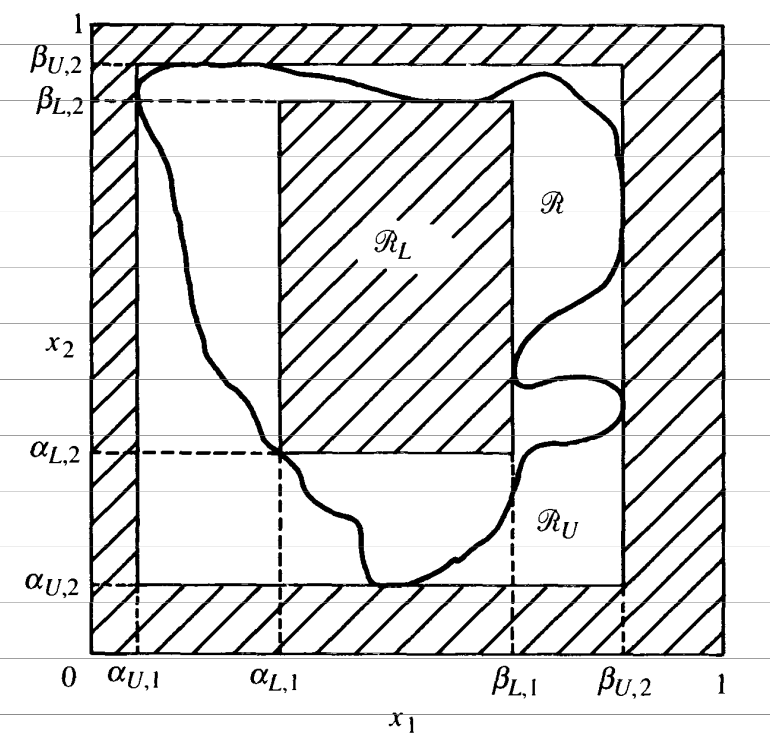
\includegraphics[width=0.7\textwidth]{images/hyperrectangle.png}
\caption{二维的矩形界:$\mathscr{R}_L \subset \mathscr{R} \subset
  \mathscr{R}_U \subset \mathscr{J}^2$。}
\label{fig::hyperrectangle2D}
\end{figure}

\begin{theorem}{}
  令
  \begin{equation}
    \Phi_L(\vec{x}) = \left\{
    \begin{array}{ll}
      1,& \vec{x} \in \mathscr{R}_L\\
      0,& \mbox{其他}.
      \end{array}
      \right.
      \label{eq::sta_L}
  \end{equation}
  和
  \begin{equation}
  \Phi_L(\vec{x}) = \left\{
  \begin{array}{ll}
    1,& \vec{x} \in \mathscr{R}_L\\
    0,& \mbox{其他}.
    \end{array}
    \right.
    \label{eq::sta_U}
  \end{equation}
  若$f(x)$表示$U(0, 1)$的PDF,令$\vec{X}$服从PDF为:
  \begin{equation}
    f(\vec{x}, \lambda_L, \lambda_U) = \frac{\phi_L(\vec{x}) -
      \phi_U(\vec{x})}{\lambda_U - \lambda_L}f(\vec{x}), \vec{x} \in
    \mathscr{J}^m.
    \label{eq::hyperrectangle_pdf}
  \end{equation}
  则
  \begin{equation}
    Z = \lambda_L + (\lambda_U - \lambda_L) \phi(\vec{X}),
    \label{eq::hyper_est}
  \end{equation}
  满足
  \begin{enumerate}
  \item
    \begin{equation}
      E[Z] = \lambda.
      \label{eq::hyper_exp}
    \end{equation}
  \item
    \begin{eqnarray}
      \mathrm{var} Z & = & (\lambda - \lambda_L)(\lambda_U - \lambda)
      \label{eq::hyper_var}
      \\
      & \leq & \frac{(\lambda_U - \lambda_L)^2}{4}. \notag
    \end{eqnarray}
  \end{enumerate}
    \label{thm::hyperrectangle}
\end{theorem}

这个定理的证明是简单的。接下去的问题如何产生服从$f(\vec{x}, \lambda_L,
\lambda_U)$的随机数?办法基本上有两种,一种是仍然产生在整个
$\mathscr{J}^m$均匀分布的点,但是用拒绝接受(AR)策略来过滤出落在
$\mathscr{R}_L$和$\mathscr{R}_U$之间的点。第二种是考虑整个
$\mathscr{R}_U \backslash \mathscr{R}_L$区域被$\alpha_{Li}$,
$\alpha_{Ui}$,$\beta_{Li}$和$\beta_{Ui}$分成了$3^m - 1$个小超矩形块。
我们当然不能逐个均匀投点(原因?)然而我们可以先从这些块中,按体积为概
率选择一个,再再上面均匀投点,这样投点的计算量仍然是$\theta(m)$的。
这两种策略的具体实现都参见参考书2.5节。
